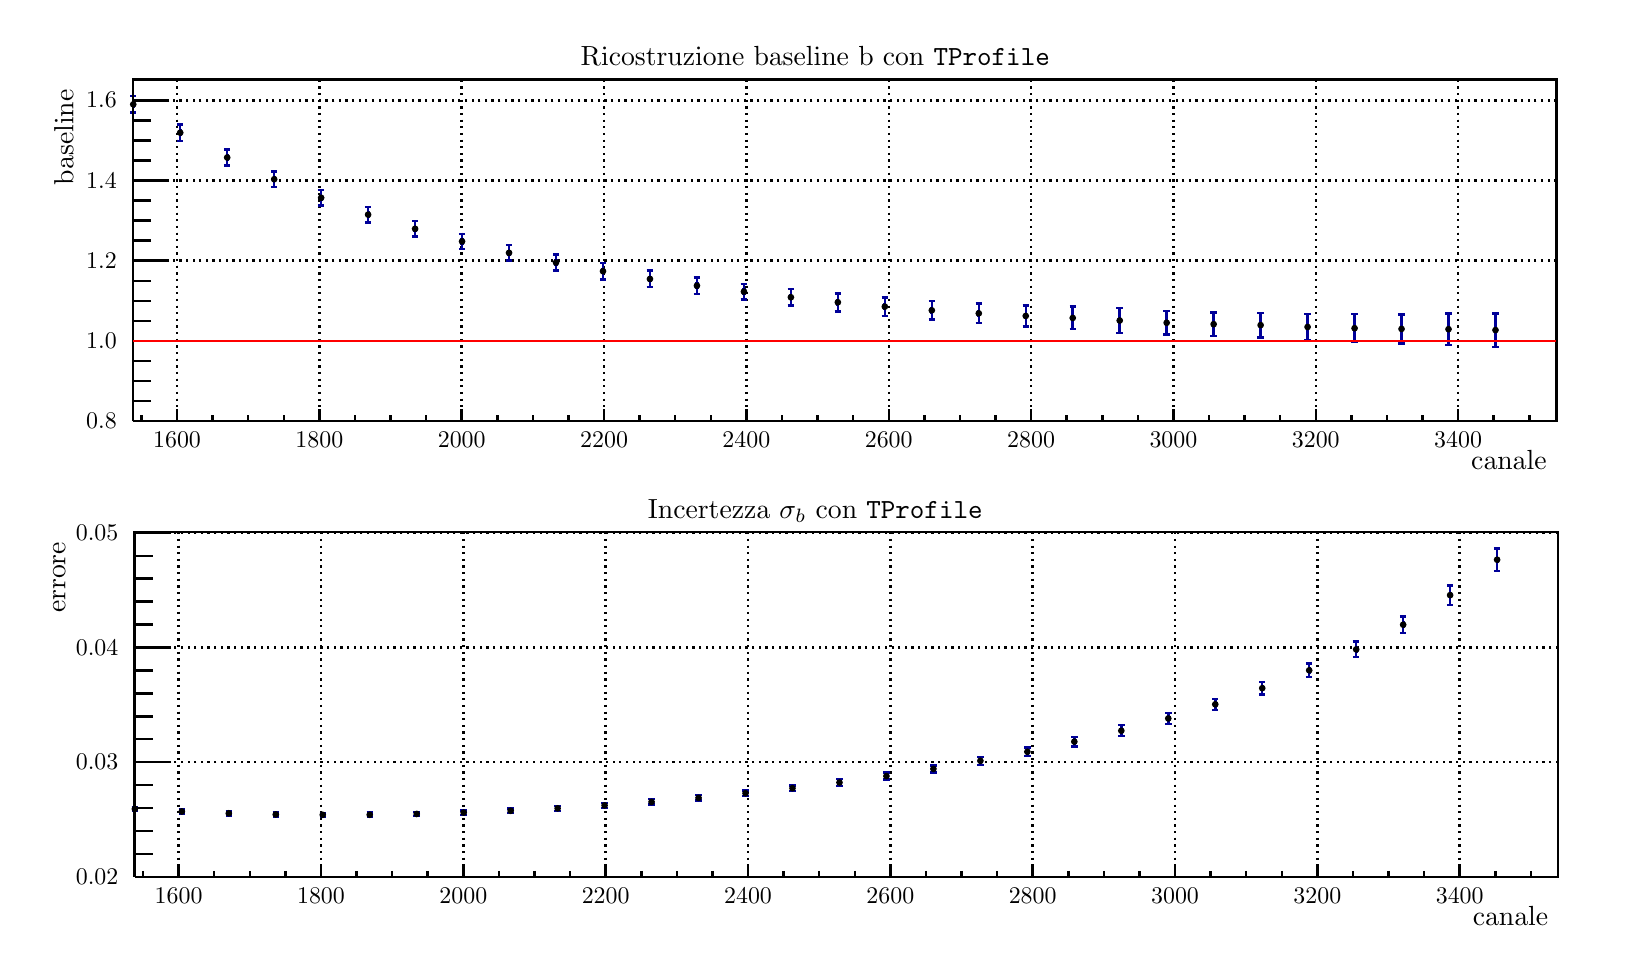
\begin{tikzpicture}
\pgfdeclareplotmark{cross} {
\pgfpathmoveto{\pgfpoint{-0.3\pgfplotmarksize}{\pgfplotmarksize}}
\pgfpathlineto{\pgfpoint{+0.3\pgfplotmarksize}{\pgfplotmarksize}}
\pgfpathlineto{\pgfpoint{+0.3\pgfplotmarksize}{0.3\pgfplotmarksize}}
\pgfpathlineto{\pgfpoint{+1\pgfplotmarksize}{0.3\pgfplotmarksize}}
\pgfpathlineto{\pgfpoint{+1\pgfplotmarksize}{-0.3\pgfplotmarksize}}
\pgfpathlineto{\pgfpoint{+0.3\pgfplotmarksize}{-0.3\pgfplotmarksize}}
\pgfpathlineto{\pgfpoint{+0.3\pgfplotmarksize}{-1.\pgfplotmarksize}}
\pgfpathlineto{\pgfpoint{-0.3\pgfplotmarksize}{-1.\pgfplotmarksize}}
\pgfpathlineto{\pgfpoint{-0.3\pgfplotmarksize}{-0.3\pgfplotmarksize}}
\pgfpathlineto{\pgfpoint{-1.\pgfplotmarksize}{-0.3\pgfplotmarksize}}
\pgfpathlineto{\pgfpoint{-1.\pgfplotmarksize}{0.3\pgfplotmarksize}}
\pgfpathlineto{\pgfpoint{-0.3\pgfplotmarksize}{0.3\pgfplotmarksize}}
\pgfpathclose
\pgfusepathqstroke
}
\pgfdeclareplotmark{cross*} {
\pgfpathmoveto{\pgfpoint{-0.3\pgfplotmarksize}{\pgfplotmarksize}}
\pgfpathlineto{\pgfpoint{+0.3\pgfplotmarksize}{\pgfplotmarksize}}
\pgfpathlineto{\pgfpoint{+0.3\pgfplotmarksize}{0.3\pgfplotmarksize}}
\pgfpathlineto{\pgfpoint{+1\pgfplotmarksize}{0.3\pgfplotmarksize}}
\pgfpathlineto{\pgfpoint{+1\pgfplotmarksize}{-0.3\pgfplotmarksize}}
\pgfpathlineto{\pgfpoint{+0.3\pgfplotmarksize}{-0.3\pgfplotmarksize}}
\pgfpathlineto{\pgfpoint{+0.3\pgfplotmarksize}{-1.\pgfplotmarksize}}
\pgfpathlineto{\pgfpoint{-0.3\pgfplotmarksize}{-1.\pgfplotmarksize}}
\pgfpathlineto{\pgfpoint{-0.3\pgfplotmarksize}{-0.3\pgfplotmarksize}}
\pgfpathlineto{\pgfpoint{-1.\pgfplotmarksize}{-0.3\pgfplotmarksize}}
\pgfpathlineto{\pgfpoint{-1.\pgfplotmarksize}{0.3\pgfplotmarksize}}
\pgfpathlineto{\pgfpoint{-0.3\pgfplotmarksize}{0.3\pgfplotmarksize}}
\pgfpathclose
\pgfusepathqfillstroke
}
\pgfdeclareplotmark{newstar} {
\pgfpathmoveto{\pgfqpoint{0pt}{\pgfplotmarksize}}
\pgfpathlineto{\pgfqpointpolar{44}{0.5\pgfplotmarksize}}
\pgfpathlineto{\pgfqpointpolar{18}{\pgfplotmarksize}}
\pgfpathlineto{\pgfqpointpolar{-20}{0.5\pgfplotmarksize}}
\pgfpathlineto{\pgfqpointpolar{-54}{\pgfplotmarksize}}
\pgfpathlineto{\pgfqpointpolar{-90}{0.5\pgfplotmarksize}}
\pgfpathlineto{\pgfqpointpolar{234}{\pgfplotmarksize}}
\pgfpathlineto{\pgfqpointpolar{198}{0.5\pgfplotmarksize}}
\pgfpathlineto{\pgfqpointpolar{162}{\pgfplotmarksize}}
\pgfpathlineto{\pgfqpointpolar{134}{0.5\pgfplotmarksize}}
\pgfpathclose
\pgfusepathqstroke
}
\pgfdeclareplotmark{newstar*} {
\pgfpathmoveto{\pgfqpoint{0pt}{\pgfplotmarksize}}
\pgfpathlineto{\pgfqpointpolar{44}{0.5\pgfplotmarksize}}
\pgfpathlineto{\pgfqpointpolar{18}{\pgfplotmarksize}}
\pgfpathlineto{\pgfqpointpolar{-20}{0.5\pgfplotmarksize}}
\pgfpathlineto{\pgfqpointpolar{-54}{\pgfplotmarksize}}
\pgfpathlineto{\pgfqpointpolar{-90}{0.5\pgfplotmarksize}}
\pgfpathlineto{\pgfqpointpolar{234}{\pgfplotmarksize}}
\pgfpathlineto{\pgfqpointpolar{198}{0.5\pgfplotmarksize}}
\pgfpathlineto{\pgfqpointpolar{162}{\pgfplotmarksize}}
\pgfpathlineto{\pgfqpointpolar{134}{0.5\pgfplotmarksize}}
\pgfpathclose
\pgfusepathqfillstroke
}
\definecolor{c}{rgb}{1,1,1};
\draw [color=c, fill=c] (0,0) rectangle (20,11.5133);
\draw [color=c, fill=c] (0.2,5.87178) rectangle (19.8,11.3982);
\draw [color=c, fill=c] (1.32924,6.52352) rectangle (19.407,10.8589);
\definecolor{c}{rgb}{0,0,0};
\draw [c,line width=0.9] (1.32924,6.52352) -- (1.32924,10.8589) -- (19.407,10.8589) -- (19.407,6.52352) -- (1.32924,6.52352);
\definecolor{c}{rgb}{1,1,1};
\draw [color=c, fill=c] (1.32924,6.52352) rectangle (19.407,10.8589);
\definecolor{c}{rgb}{0,0,0};
\draw [c,line width=0.9] (1.32924,6.52352) -- (1.32924,10.8589) -- (19.407,10.8589) -- (19.407,6.52352) -- (1.32924,6.52352);
\draw [c,line width=0.9] (1.32924,6.52352) -- (19.407,6.52352);
\draw [c,dash pattern=on 0.80pt off 1.60pt ,line width=0.9] (1.88965,10.8589) -- (1.88965,6.52352);
\draw [c,dash pattern=on 0.80pt off 1.60pt ,line width=0.9] (3.69742,10.8589) -- (3.69742,6.52352);
\draw [c,dash pattern=on 0.80pt off 1.60pt ,line width=0.9] (5.50519,10.8589) -- (5.50519,6.52352);
\draw [c,dash pattern=on 0.80pt off 1.60pt ,line width=0.9] (7.31297,10.8589) -- (7.31297,6.52352);
\draw [c,dash pattern=on 0.80pt off 1.60pt ,line width=0.9] (9.12074,10.8589) -- (9.12074,6.52352);
\draw [c,dash pattern=on 0.80pt off 1.60pt ,line width=0.9] (10.9285,10.8589) -- (10.9285,6.52352);
\draw [c,dash pattern=on 0.80pt off 1.60pt ,line width=0.9] (12.7363,10.8589) -- (12.7363,6.52352);
\draw [c,dash pattern=on 0.80pt off 1.60pt ,line width=0.9] (14.544,10.8589) -- (14.544,6.52352);
\draw [c,dash pattern=on 0.80pt off 1.60pt ,line width=0.9] (16.3518,10.8589) -- (16.3518,6.52352);
\draw [c,dash pattern=on 0.80pt off 1.60pt ,line width=0.9] (18.1596,10.8589) -- (18.1596,6.52352);
\draw [c,dash pattern=on 0.80pt off 1.60pt ,line width=0.9] (1.88965,10.8589) -- (1.88965,6.52352);
\draw [c,dash pattern=on 0.80pt off 1.60pt ,line width=0.9] (18.1596,10.8589) -- (18.1596,6.52352);
\draw [c,line width=0.9] (1.32924,6.52352) -- (1.32924,10.8589);
\draw [c,dash pattern=on 0.80pt off 1.60pt ,line width=0.9] (19.407,6.52352) -- (1.32924,6.52352);
\draw [c,dash pattern=on 0.80pt off 1.60pt ,line width=0.9] (19.407,7.54218) -- (1.32924,7.54218);
\draw [c,dash pattern=on 0.80pt off 1.60pt ,line width=0.9] (19.407,8.56083) -- (1.32924,8.56083);
\draw [c,dash pattern=on 0.80pt off 1.60pt ,line width=0.9] (19.407,9.57949) -- (1.32924,9.57949);
\draw [c,dash pattern=on 0.80pt off 1.60pt ,line width=0.9] (19.407,10.5982) -- (1.32924,10.5982);
\draw [c,dash pattern=on 0.80pt off 1.60pt ,line width=0.9] (19.407,10.5982) -- (1.32924,10.5982);
\definecolor{c}{rgb}{0,0,0.6};
\draw [c,line width=0.9] (1.33376,10.4404) -- (1.33376,10.5464);
\draw [c,line width=0.9] (1.33376,10.5464) -- (1.33376,10.6524);
\draw [c,line width=0.9] (1.32924,10.5464) -- (1.33376,10.5464);
\draw [c,line width=0.9] (1.33376,10.5464) -- (1.33828,10.5464);
\draw [c,line width=0.9] (1.29286,10.4404) -- (1.37466,10.4404);
\draw [c,line width=0.9] (1.29286,10.6524) -- (1.37466,10.6524);
\draw [c,line width=0.9] (1.32924,10.5055) -- (1.32924,10.5873);
\draw [c,line width=0.9] (1.33828,10.5055) -- (1.33828,10.5873);
\definecolor{c}{rgb}{0,0,0};
\foreach \P in {(1.33376,10.5464)}{\draw[mark options={color=c,fill=c},mark size=2.402402pt,mark=*,mark size=1pt] plot coordinates {\P};}
\definecolor{c}{rgb}{0,0,0.6};
\draw [c,line width=0.9] (1.93033,10.0814) -- (1.93033,10.1865);
\draw [c,line width=0.9] (1.93033,10.1865) -- (1.93033,10.2915);
\draw [c,line width=0.9] (1.92581,10.1865) -- (1.93033,10.1865);
\draw [c,line width=0.9] (1.93033,10.1865) -- (1.93485,10.1865);
\draw [c,line width=0.9] (1.88943,10.0814) -- (1.97123,10.0814);
\draw [c,line width=0.9] (1.88943,10.2915) -- (1.97123,10.2915);
\draw [c,line width=0.9] (1.92581,10.1456) -- (1.92581,10.2274);
\draw [c,line width=0.9] (1.93485,10.1456) -- (1.93485,10.2274);
\definecolor{c}{rgb}{0,0,0};
\foreach \P in {(1.93033,10.1865)}{\draw[mark options={color=c,fill=c},mark size=2.402402pt,mark=*,mark size=1pt] plot coordinates {\P};}
\definecolor{c}{rgb}{0,0,0.6};
\draw [c,line width=0.9] (2.52689,9.77198) -- (2.52689,9.87129);
\draw [c,line width=0.9] (2.52689,9.87129) -- (2.52689,9.9706);
\draw [c,line width=0.9] (2.52237,9.87129) -- (2.52689,9.87129);
\draw [c,line width=0.9] (2.52689,9.87129) -- (2.53141,9.87129);
\draw [c,line width=0.9] (2.48599,9.77198) -- (2.56779,9.77198);
\draw [c,line width=0.9] (2.48599,9.9706) -- (2.56779,9.9706);
\draw [c,line width=0.9] (2.52237,9.83039) -- (2.52237,9.91219);
\draw [c,line width=0.9] (2.53141,9.83039) -- (2.53141,9.91219);
\definecolor{c}{rgb}{0,0,0};
\foreach \P in {(2.52689,9.87129)}{\draw[mark options={color=c,fill=c},mark size=2.402402pt,mark=*,mark size=1pt] plot coordinates {\P};}
\definecolor{c}{rgb}{0,0,0.6};
\draw [c,line width=0.9] (3.12346,9.49474) -- (3.12346,9.59535);
\draw [c,line width=0.9] (3.12346,9.59535) -- (3.12346,9.69596);
\draw [c,line width=0.9] (3.11894,9.59535) -- (3.12346,9.59535);
\draw [c,line width=0.9] (3.12346,9.59535) -- (3.12798,9.59535);
\draw [c,line width=0.9] (3.08256,9.49474) -- (3.16436,9.49474);
\draw [c,line width=0.9] (3.08256,9.69596) -- (3.16436,9.69596);
\draw [c,line width=0.9] (3.11894,9.55445) -- (3.11894,9.63625);
\draw [c,line width=0.9] (3.12798,9.55445) -- (3.12798,9.63625);
\definecolor{c}{rgb}{0,0,0};
\foreach \P in {(3.12346,9.59535)}{\draw[mark options={color=c,fill=c},mark size=2.402402pt,mark=*,mark size=1pt] plot coordinates {\P};}
\definecolor{c}{rgb}{0,0,0.6};
\draw [c,line width=0.9] (3.72002,9.26345) -- (3.72002,9.36015);
\draw [c,line width=0.9] (3.72002,9.36015) -- (3.72002,9.45685);
\draw [c,line width=0.9] (3.7155,9.36015) -- (3.72002,9.36015);
\draw [c,line width=0.9] (3.72002,9.36015) -- (3.72454,9.36015);
\draw [c,line width=0.9] (3.67912,9.26345) -- (3.76092,9.26345);
\draw [c,line width=0.9] (3.67912,9.45685) -- (3.76092,9.45685);
\draw [c,line width=0.9] (3.7155,9.31925) -- (3.7155,9.40105);
\draw [c,line width=0.9] (3.72454,9.31925) -- (3.72454,9.40105);
\definecolor{c}{rgb}{0,0,0};
\foreach \P in {(3.72002,9.36015)}{\draw[mark options={color=c,fill=c},mark size=2.402402pt,mark=*,mark size=1pt] plot coordinates {\P};}
\definecolor{c}{rgb}{0,0,0.6};
\draw [c,line width=0.9] (4.31659,9.04754) -- (4.31659,9.14585);
\draw [c,line width=0.9] (4.31659,9.14585) -- (4.31659,9.24417);
\draw [c,line width=0.9] (4.31207,9.14585) -- (4.31659,9.14585);
\draw [c,line width=0.9] (4.31659,9.14585) -- (4.3211,9.14585);
\draw [c,line width=0.9] (4.27569,9.04754) -- (4.35748,9.04754);
\draw [c,line width=0.9] (4.27569,9.24417) -- (4.35748,9.24417);
\draw [c,line width=0.9] (4.31207,9.10495) -- (4.31207,9.18675);
\draw [c,line width=0.9] (4.3211,9.10495) -- (4.3211,9.18675);
\definecolor{c}{rgb}{0,0,0};
\foreach \P in {(4.31659,9.14585)}{\draw[mark options={color=c,fill=c},mark size=2.402402pt,mark=*,mark size=1pt] plot coordinates {\P};}
\definecolor{c}{rgb}{0,0,0.6};
\draw [c,line width=0.9] (4.91315,8.86903) -- (4.91315,8.96597);
\draw [c,line width=0.9] (4.91315,8.96597) -- (4.91315,9.0629);
\draw [c,line width=0.9] (4.90863,8.96597) -- (4.91315,8.96597);
\draw [c,line width=0.9] (4.91315,8.96597) -- (4.91767,8.96597);
\draw [c,line width=0.9] (4.87225,8.86903) -- (4.95405,8.86903);
\draw [c,line width=0.9] (4.87225,9.0629) -- (4.95405,9.0629);
\draw [c,line width=0.9] (4.90863,8.92507) -- (4.90863,9.00687);
\draw [c,line width=0.9] (4.91767,8.92507) -- (4.91767,9.00687);
\definecolor{c}{rgb}{0,0,0};
\foreach \P in {(4.91315,8.96597)}{\draw[mark options={color=c,fill=c},mark size=2.402402pt,mark=*,mark size=1pt] plot coordinates {\P};}
\definecolor{c}{rgb}{0,0,0.6};
\draw [c,line width=0.9] (5.50971,8.71081) -- (5.50971,8.80571);
\draw [c,line width=0.9] (5.50971,8.80571) -- (5.50971,8.9006);
\draw [c,line width=0.9] (5.50519,8.80571) -- (5.50971,8.80571);
\draw [c,line width=0.9] (5.50971,8.80571) -- (5.51423,8.80571);
\draw [c,line width=0.9] (5.46881,8.71081) -- (5.55061,8.71081);
\draw [c,line width=0.9] (5.46881,8.9006) -- (5.55061,8.9006);
\draw [c,line width=0.9] (5.50519,8.76481) -- (5.50519,8.84661);
\draw [c,line width=0.9] (5.51423,8.76481) -- (5.51423,8.84661);
\definecolor{c}{rgb}{0,0,0};
\foreach \P in {(5.50971,8.80571)}{\draw[mark options={color=c,fill=c},mark size=2.402402pt,mark=*,mark size=1pt] plot coordinates {\P};}
\definecolor{c}{rgb}{0,0,0.6};
\draw [c,line width=0.9] (6.10628,8.5644) -- (6.10628,8.6607);
\draw [c,line width=0.9] (6.10628,8.6607) -- (6.10628,8.757);
\draw [c,line width=0.9] (6.10176,8.6607) -- (6.10628,8.6607);
\draw [c,line width=0.9] (6.10628,8.6607) -- (6.1108,8.6607);
\draw [c,line width=0.9] (6.06538,8.5644) -- (6.14718,8.5644);
\draw [c,line width=0.9] (6.06538,8.757) -- (6.14718,8.757);
\draw [c,line width=0.9] (6.10176,8.6198) -- (6.10176,8.7016);
\draw [c,line width=0.9] (6.1108,8.6198) -- (6.1108,8.7016);
\definecolor{c}{rgb}{0,0,0};
\foreach \P in {(6.10628,8.6607)}{\draw[mark options={color=c,fill=c},mark size=2.402402pt,mark=*,mark size=1pt] plot coordinates {\P};}
\definecolor{c}{rgb}{0,0,0.6};
\draw [c,line width=0.9] (6.70284,8.43674) -- (6.70284,8.53694);
\draw [c,line width=0.9] (6.70284,8.53694) -- (6.70284,8.63714);
\draw [c,line width=0.9] (6.69832,8.53694) -- (6.70284,8.53694);
\draw [c,line width=0.9] (6.70284,8.53694) -- (6.70736,8.53694);
\draw [c,line width=0.9] (6.66194,8.43674) -- (6.74374,8.43674);
\draw [c,line width=0.9] (6.66194,8.63714) -- (6.74374,8.63714);
\draw [c,line width=0.9] (6.69832,8.49605) -- (6.69832,8.57784);
\draw [c,line width=0.9] (6.70736,8.49605) -- (6.70736,8.57784);
\definecolor{c}{rgb}{0,0,0};
\foreach \P in {(6.70284,8.53694)}{\draw[mark options={color=c,fill=c},mark size=2.402402pt,mark=*,mark size=1pt] plot coordinates {\P};}
\definecolor{c}{rgb}{0,0,0.6};
\draw [c,line width=0.9] (7.29941,8.32287) -- (7.29941,8.4275);
\draw [c,line width=0.9] (7.29941,8.4275) -- (7.29941,8.53213);
\draw [c,line width=0.9] (7.29489,8.4275) -- (7.29941,8.4275);
\draw [c,line width=0.9] (7.29941,8.4275) -- (7.30393,8.4275);
\draw [c,line width=0.9] (7.25851,8.32287) -- (7.34031,8.32287);
\draw [c,line width=0.9] (7.25851,8.53213) -- (7.34031,8.53213);
\draw [c,line width=0.9] (7.29489,8.3866) -- (7.29489,8.4684);
\draw [c,line width=0.9] (7.30393,8.3866) -- (7.30393,8.4684);
\definecolor{c}{rgb}{0,0,0};
\foreach \P in {(7.29941,8.4275)}{\draw[mark options={color=c,fill=c},mark size=2.402402pt,mark=*,mark size=1pt] plot coordinates {\P};}
\definecolor{c}{rgb}{0,0,0.6};
\draw [c,line width=0.9] (7.89597,8.22387) -- (7.89597,8.32903);
\draw [c,line width=0.9] (7.89597,8.32903) -- (7.89597,8.43419);
\draw [c,line width=0.9] (7.89145,8.32903) -- (7.89597,8.32903);
\draw [c,line width=0.9] (7.89597,8.32903) -- (7.90049,8.32903);
\draw [c,line width=0.9] (7.85507,8.22387) -- (7.93687,8.22387);
\draw [c,line width=0.9] (7.85507,8.43419) -- (7.93687,8.43419);
\draw [c,line width=0.9] (7.89145,8.28813) -- (7.89145,8.36993);
\draw [c,line width=0.9] (7.90049,8.28813) -- (7.90049,8.36993);
\definecolor{c}{rgb}{0,0,0};
\foreach \P in {(7.89597,8.32903)}{\draw[mark options={color=c,fill=c},mark size=2.402402pt,mark=*,mark size=1pt] plot coordinates {\P};}
\definecolor{c}{rgb}{0,0,0.6};
\draw [c,line width=0.9] (8.49254,8.14082) -- (8.49254,8.24346);
\draw [c,line width=0.9] (8.49254,8.24346) -- (8.49254,8.34609);
\draw [c,line width=0.9] (8.48802,8.24346) -- (8.49254,8.24346);
\draw [c,line width=0.9] (8.49254,8.24346) -- (8.49706,8.24346);
\draw [c,line width=0.9] (8.45164,8.14082) -- (8.53344,8.14082);
\draw [c,line width=0.9] (8.45164,8.34609) -- (8.53344,8.34609);
\draw [c,line width=0.9] (8.48802,8.20256) -- (8.48802,8.28436);
\draw [c,line width=0.9] (8.49706,8.20256) -- (8.49706,8.28436);
\definecolor{c}{rgb}{0,0,0};
\foreach \P in {(8.49254,8.24346)}{\draw[mark options={color=c,fill=c},mark size=2.402402pt,mark=*,mark size=1pt] plot coordinates {\P};}
\definecolor{c}{rgb}{0,0,0.6};
\draw [c,line width=0.9] (9.0891,8.06816) -- (9.0891,8.16813);
\draw [c,line width=0.9] (9.0891,8.16813) -- (9.0891,8.2681);
\draw [c,line width=0.9] (9.08458,8.16813) -- (9.0891,8.16813);
\draw [c,line width=0.9] (9.0891,8.16813) -- (9.09362,8.16813);
\draw [c,line width=0.9] (9.0482,8.06816) -- (9.13,8.06816);
\draw [c,line width=0.9] (9.0482,8.2681) -- (9.13,8.2681);
\draw [c,line width=0.9] (9.08458,8.12723) -- (9.08458,8.20903);
\draw [c,line width=0.9] (9.09362,8.12723) -- (9.09362,8.20903);
\definecolor{c}{rgb}{0,0,0};
\foreach \P in {(9.0891,8.16813)}{\draw[mark options={color=c,fill=c},mark size=2.402402pt,mark=*,mark size=1pt] plot coordinates {\P};}
\definecolor{c}{rgb}{0,0,0.6};
\draw [c,line width=0.9] (9.68566,7.99221) -- (9.68566,8.0965);
\draw [c,line width=0.9] (9.68566,8.0965) -- (9.68566,8.20079);
\draw [c,line width=0.9] (9.68115,8.0965) -- (9.68566,8.0965);
\draw [c,line width=0.9] (9.68566,8.0965) -- (9.69018,8.0965);
\draw [c,line width=0.9] (9.64476,7.99221) -- (9.72656,7.99221);
\draw [c,line width=0.9] (9.64476,8.20079) -- (9.72656,8.20079);
\draw [c,line width=0.9] (9.68115,8.0556) -- (9.68115,8.1374);
\draw [c,line width=0.9] (9.69018,8.0556) -- (9.69018,8.1374);
\definecolor{c}{rgb}{0,0,0};
\foreach \P in {(9.68566,8.0965)}{\draw[mark options={color=c,fill=c},mark size=2.402402pt,mark=*,mark size=1pt] plot coordinates {\P};}
\definecolor{c}{rgb}{0,0,0.6};
\draw [c,line width=0.9] (10.2822,7.9187) -- (10.2822,8.03262);
\draw [c,line width=0.9] (10.2822,8.03262) -- (10.2822,8.14655);
\draw [c,line width=0.9] (10.2777,8.03262) -- (10.2822,8.03262);
\draw [c,line width=0.9] (10.2822,8.03262) -- (10.2867,8.03262);
\draw [c,line width=0.9] (10.2413,7.9187) -- (10.3231,7.9187);
\draw [c,line width=0.9] (10.2413,8.14655) -- (10.3231,8.14655);
\draw [c,line width=0.9] (10.2777,7.99172) -- (10.2777,8.07352);
\draw [c,line width=0.9] (10.2867,7.99172) -- (10.2867,8.07352);
\definecolor{c}{rgb}{0,0,0};
\foreach \P in {(10.2822,8.03262)}{\draw[mark options={color=c,fill=c},mark size=2.402402pt,mark=*,mark size=1pt] plot coordinates {\P};}
\definecolor{c}{rgb}{0,0,0.6};
\draw [c,line width=0.9] (10.8788,7.86112) -- (10.8788,7.97751);
\draw [c,line width=0.9] (10.8788,7.97751) -- (10.8788,8.09391);
\draw [c,line width=0.9] (10.8743,7.97751) -- (10.8788,7.97751);
\draw [c,line width=0.9] (10.8788,7.97751) -- (10.8833,7.97751);
\draw [c,line width=0.9] (10.8379,7.86112) -- (10.9197,7.86112);
\draw [c,line width=0.9] (10.8379,8.09391) -- (10.9197,8.09391);
\draw [c,line width=0.9] (10.8743,7.93661) -- (10.8743,8.01841);
\draw [c,line width=0.9] (10.8833,7.93661) -- (10.8833,8.01841);
\definecolor{c}{rgb}{0,0,0};
\foreach \P in {(10.8788,7.97751)}{\draw[mark options={color=c,fill=c},mark size=2.402402pt,mark=*,mark size=1pt] plot coordinates {\P};}
\definecolor{c}{rgb}{0,0,0.6};
\draw [c,line width=0.9] (11.4754,7.81342) -- (11.4754,7.93035);
\draw [c,line width=0.9] (11.4754,7.93035) -- (11.4754,8.04729);
\draw [c,line width=0.9] (11.4708,7.93035) -- (11.4754,7.93035);
\draw [c,line width=0.9] (11.4754,7.93035) -- (11.4799,7.93035);
\draw [c,line width=0.9] (11.4345,7.81342) -- (11.5163,7.81342);
\draw [c,line width=0.9] (11.4345,8.04729) -- (11.5163,8.04729);
\draw [c,line width=0.9] (11.4708,7.88945) -- (11.4708,7.97125);
\draw [c,line width=0.9] (11.4799,7.88945) -- (11.4799,7.97125);
\definecolor{c}{rgb}{0,0,0};
\foreach \P in {(11.4754,7.93035)}{\draw[mark options={color=c,fill=c},mark size=2.402402pt,mark=*,mark size=1pt] plot coordinates {\P};}
\definecolor{c}{rgb}{0,0,0.6};
\draw [c,line width=0.9] (12.0719,7.76776) -- (12.0719,7.89226);
\draw [c,line width=0.9] (12.0719,7.89226) -- (12.0719,8.01675);
\draw [c,line width=0.9] (12.0674,7.89226) -- (12.0719,7.89226);
\draw [c,line width=0.9] (12.0719,7.89226) -- (12.0764,7.89226);
\draw [c,line width=0.9] (12.031,7.76776) -- (12.1128,7.76776);
\draw [c,line width=0.9] (12.031,8.01675) -- (12.1128,8.01675);
\draw [c,line width=0.9] (12.0674,7.85136) -- (12.0674,7.93316);
\draw [c,line width=0.9] (12.0764,7.85136) -- (12.0764,7.93316);
\definecolor{c}{rgb}{0,0,0};
\foreach \P in {(12.0719,7.89226)}{\draw[mark options={color=c,fill=c},mark size=2.402402pt,mark=*,mark size=1pt] plot coordinates {\P};}
\definecolor{c}{rgb}{0,0,0.6};
\draw [c,line width=0.9] (12.6685,7.7248) -- (12.6685,7.85916);
\draw [c,line width=0.9] (12.6685,7.85916) -- (12.6685,7.99353);
\draw [c,line width=0.9] (12.664,7.85916) -- (12.6685,7.85916);
\draw [c,line width=0.9] (12.6685,7.85916) -- (12.673,7.85916);
\draw [c,line width=0.9] (12.6276,7.7248) -- (12.7094,7.7248);
\draw [c,line width=0.9] (12.6276,7.99353) -- (12.7094,7.99353);
\draw [c,line width=0.9] (12.664,7.81826) -- (12.664,7.90006);
\draw [c,line width=0.9] (12.673,7.81826) -- (12.673,7.90006);
\definecolor{c}{rgb}{0,0,0};
\foreach \P in {(12.6685,7.85916)}{\draw[mark options={color=c,fill=c},mark size=2.402402pt,mark=*,mark size=1pt] plot coordinates {\P};}
\definecolor{c}{rgb}{0,0,0.6};
\draw [c,line width=0.9] (13.2651,7.69038) -- (13.2651,7.83369);
\draw [c,line width=0.9] (13.2651,7.83369) -- (13.2651,7.977);
\draw [c,line width=0.9] (13.2605,7.83369) -- (13.2651,7.83369);
\draw [c,line width=0.9] (13.2651,7.83369) -- (13.2696,7.83369);
\draw [c,line width=0.9] (13.2242,7.69038) -- (13.306,7.69038);
\draw [c,line width=0.9] (13.2242,7.977) -- (13.306,7.977);
\draw [c,line width=0.9] (13.2605,7.79279) -- (13.2605,7.87459);
\draw [c,line width=0.9] (13.2696,7.79279) -- (13.2696,7.87459);
\definecolor{c}{rgb}{0,0,0};
\foreach \P in {(13.2651,7.83369)}{\draw[mark options={color=c,fill=c},mark size=2.402402pt,mark=*,mark size=1pt] plot coordinates {\P};}
\definecolor{c}{rgb}{0,0,0.6};
\draw [c,line width=0.9] (13.8616,7.64494) -- (13.8616,7.8011);
\draw [c,line width=0.9] (13.8616,7.8011) -- (13.8616,7.95725);
\draw [c,line width=0.9] (13.8571,7.8011) -- (13.8616,7.8011);
\draw [c,line width=0.9] (13.8616,7.8011) -- (13.8661,7.8011);
\draw [c,line width=0.9] (13.8207,7.64494) -- (13.9025,7.64494);
\draw [c,line width=0.9] (13.8207,7.95725) -- (13.9025,7.95725);
\draw [c,line width=0.9] (13.8571,7.7602) -- (13.8571,7.842);
\draw [c,line width=0.9] (13.8661,7.7602) -- (13.8661,7.842);
\definecolor{c}{rgb}{0,0,0};
\foreach \P in {(13.8616,7.8011)}{\draw[mark options={color=c,fill=c},mark size=2.402402pt,mark=*,mark size=1pt] plot coordinates {\P};}
\definecolor{c}{rgb}{0,0,0.6};
\draw [c,line width=0.9] (14.4582,7.62508) -- (14.4582,7.77248);
\draw [c,line width=0.9] (14.4582,7.77248) -- (14.4582,7.91988);
\draw [c,line width=0.9] (14.4537,7.77248) -- (14.4582,7.77248);
\draw [c,line width=0.9] (14.4582,7.77248) -- (14.4627,7.77248);
\draw [c,line width=0.9] (14.4173,7.62508) -- (14.4991,7.62508);
\draw [c,line width=0.9] (14.4173,7.91988) -- (14.4991,7.91988);
\draw [c,line width=0.9] (14.4537,7.73158) -- (14.4537,7.81338);
\draw [c,line width=0.9] (14.4627,7.73158) -- (14.4627,7.81338);
\definecolor{c}{rgb}{0,0,0};
\foreach \P in {(14.4582,7.77248)}{\draw[mark options={color=c,fill=c},mark size=2.402402pt,mark=*,mark size=1pt] plot coordinates {\P};}
\definecolor{c}{rgb}{0,0,0.6};
\draw [c,line width=0.9] (15.0547,7.60766) -- (15.0547,7.75437);
\draw [c,line width=0.9] (15.0547,7.75437) -- (15.0547,7.90107);
\draw [c,line width=0.9] (15.0502,7.75437) -- (15.0547,7.75437);
\draw [c,line width=0.9] (15.0547,7.75437) -- (15.0593,7.75437);
\draw [c,line width=0.9] (15.0138,7.60766) -- (15.0956,7.60766);
\draw [c,line width=0.9] (15.0138,7.90107) -- (15.0956,7.90107);
\draw [c,line width=0.9] (15.0502,7.71347) -- (15.0502,7.79527);
\draw [c,line width=0.9] (15.0593,7.71347) -- (15.0593,7.79527);
\definecolor{c}{rgb}{0,0,0};
\foreach \P in {(15.0547,7.75437)}{\draw[mark options={color=c,fill=c},mark size=2.402402pt,mark=*,mark size=1pt] plot coordinates {\P};}
\definecolor{c}{rgb}{0,0,0.6};
\draw [c,line width=0.9] (15.6513,7.58789) -- (15.6513,7.74297);
\draw [c,line width=0.9] (15.6513,7.74297) -- (15.6513,7.89804);
\draw [c,line width=0.9] (15.6468,7.74297) -- (15.6513,7.74297);
\draw [c,line width=0.9] (15.6513,7.74297) -- (15.6558,7.74297);
\draw [c,line width=0.9] (15.6104,7.58789) -- (15.6922,7.58789);
\draw [c,line width=0.9] (15.6104,7.89804) -- (15.6922,7.89804);
\draw [c,line width=0.9] (15.6468,7.70207) -- (15.6468,7.78387);
\draw [c,line width=0.9] (15.6558,7.70207) -- (15.6558,7.78387);
\definecolor{c}{rgb}{0,0,0};
\foreach \P in {(15.6513,7.74297)}{\draw[mark options={color=c,fill=c},mark size=2.402402pt,mark=*,mark size=1pt] plot coordinates {\P};}
\definecolor{c}{rgb}{0,0,0.6};
\draw [c,line width=0.9] (16.2479,7.55647) -- (16.2479,7.71907);
\draw [c,line width=0.9] (16.2479,7.71907) -- (16.2479,7.88167);
\draw [c,line width=0.9] (16.2434,7.71907) -- (16.2479,7.71907);
\draw [c,line width=0.9] (16.2479,7.71907) -- (16.2524,7.71907);
\draw [c,line width=0.9] (16.207,7.55647) -- (16.2888,7.55647);
\draw [c,line width=0.9] (16.207,7.88167) -- (16.2888,7.88167);
\draw [c,line width=0.9] (16.2434,7.67817) -- (16.2434,7.75997);
\draw [c,line width=0.9] (16.2524,7.67817) -- (16.2524,7.75997);
\definecolor{c}{rgb}{0,0,0};
\foreach \P in {(16.2479,7.71907)}{\draw[mark options={color=c,fill=c},mark size=2.402402pt,mark=*,mark size=1pt] plot coordinates {\P};}
\definecolor{c}{rgb}{0,0,0.6};
\draw [c,line width=0.9] (16.8444,7.52586) -- (16.8444,7.70343);
\draw [c,line width=0.9] (16.8444,7.70343) -- (16.8444,7.881);
\draw [c,line width=0.9] (16.8399,7.70343) -- (16.8444,7.70343);
\draw [c,line width=0.9] (16.8444,7.70343) -- (16.849,7.70343);
\draw [c,line width=0.9] (16.8035,7.52586) -- (16.8853,7.52586);
\draw [c,line width=0.9] (16.8035,7.881) -- (16.8853,7.881);
\draw [c,line width=0.9] (16.8399,7.66253) -- (16.8399,7.74433);
\draw [c,line width=0.9] (16.849,7.66253) -- (16.849,7.74433);
\definecolor{c}{rgb}{0,0,0};
\foreach \P in {(16.8444,7.70343)}{\draw[mark options={color=c,fill=c},mark size=2.402402pt,mark=*,mark size=1pt] plot coordinates {\P};}
\definecolor{c}{rgb}{0,0,0.6};
\draw [c,line width=0.9] (17.441,7.5122) -- (17.441,7.69435);
\draw [c,line width=0.9] (17.441,7.69435) -- (17.441,7.8765);
\draw [c,line width=0.9] (17.4365,7.69435) -- (17.441,7.69435);
\draw [c,line width=0.9] (17.441,7.69435) -- (17.4455,7.69435);
\draw [c,line width=0.9] (17.4001,7.5122) -- (17.4819,7.5122);
\draw [c,line width=0.9] (17.4001,7.8765) -- (17.4819,7.8765);
\draw [c,line width=0.9] (17.4365,7.65345) -- (17.4365,7.73525);
\draw [c,line width=0.9] (17.4455,7.65345) -- (17.4455,7.73525);
\definecolor{c}{rgb}{0,0,0};
\foreach \P in {(17.441,7.69435)}{\draw[mark options={color=c,fill=c},mark size=2.402402pt,mark=*,mark size=1pt] plot coordinates {\P};}
\definecolor{c}{rgb}{0,0,0.6};
\draw [c,line width=0.9] (18.0376,7.49142) -- (18.0376,7.69102);
\draw [c,line width=0.9] (18.0376,7.69102) -- (18.0376,7.89063);
\draw [c,line width=0.9] (18.033,7.69102) -- (18.0376,7.69102);
\draw [c,line width=0.9] (18.0376,7.69102) -- (18.0421,7.69102);
\draw [c,line width=0.9] (17.9967,7.49142) -- (18.0785,7.49142);
\draw [c,line width=0.9] (17.9967,7.89063) -- (18.0785,7.89063);
\draw [c,line width=0.9] (18.033,7.65012) -- (18.033,7.73192);
\draw [c,line width=0.9] (18.0421,7.65012) -- (18.0421,7.73192);
\definecolor{c}{rgb}{0,0,0};
\foreach \P in {(18.0376,7.69102)}{\draw[mark options={color=c,fill=c},mark size=2.402402pt,mark=*,mark size=1pt] plot coordinates {\P};}
\definecolor{c}{rgb}{0,0,0.6};
\draw [c,line width=0.9] (18.6341,7.46716) -- (18.6341,7.6794);
\draw [c,line width=0.9] (18.6341,7.6794) -- (18.6341,7.89164);
\draw [c,line width=0.9] (18.6296,7.6794) -- (18.6341,7.6794);
\draw [c,line width=0.9] (18.6341,7.6794) -- (18.6387,7.6794);
\draw [c,line width=0.9] (18.5932,7.46716) -- (18.675,7.46716);
\draw [c,line width=0.9] (18.5932,7.89164) -- (18.675,7.89164);
\draw [c,line width=0.9] (18.6296,7.6385) -- (18.6296,7.7203);
\draw [c,line width=0.9] (18.6387,7.6385) -- (18.6387,7.7203);
\definecolor{c}{rgb}{0,0,0};
\foreach \P in {(18.6341,7.6794)}{\draw[mark options={color=c,fill=c},mark size=2.402402pt,mark=*,mark size=1pt] plot coordinates {\P};}
\draw [c,line width=0.9] (1.32924,6.52352) -- (19.407,6.52352);
\draw [anchor= east] (19.407,6.02835) node[scale=1.0001, color=c, rotate=0]{canale};
\draw [c,line width=0.9] (1.88965,6.67643) -- (1.88965,6.52352);
\draw [c,line width=0.9] (2.3416,6.59997) -- (2.3416,6.52352);
\draw [c,line width=0.9] (2.79354,6.59997) -- (2.79354,6.52352);
\draw [c,line width=0.9] (3.24548,6.59997) -- (3.24548,6.52352);
\draw [c,line width=0.9] (3.69742,6.67643) -- (3.69742,6.52352);
\draw [c,line width=0.9] (4.14937,6.59997) -- (4.14937,6.52352);
\draw [c,line width=0.9] (4.60131,6.59997) -- (4.60131,6.52352);
\draw [c,line width=0.9] (5.05325,6.59997) -- (5.05325,6.52352);
\draw [c,line width=0.9] (5.50519,6.67643) -- (5.50519,6.52352);
\draw [c,line width=0.9] (5.95714,6.59997) -- (5.95714,6.52352);
\draw [c,line width=0.9] (6.40908,6.59997) -- (6.40908,6.52352);
\draw [c,line width=0.9] (6.86102,6.59997) -- (6.86102,6.52352);
\draw [c,line width=0.9] (7.31297,6.67643) -- (7.31297,6.52352);
\draw [c,line width=0.9] (7.76491,6.59997) -- (7.76491,6.52352);
\draw [c,line width=0.9] (8.21685,6.59997) -- (8.21685,6.52352);
\draw [c,line width=0.9] (8.66879,6.59997) -- (8.66879,6.52352);
\draw [c,line width=0.9] (9.12074,6.67643) -- (9.12074,6.52352);
\draw [c,line width=0.9] (9.57268,6.59997) -- (9.57268,6.52352);
\draw [c,line width=0.9] (10.0246,6.59997) -- (10.0246,6.52352);
\draw [c,line width=0.9] (10.4766,6.59997) -- (10.4766,6.52352);
\draw [c,line width=0.9] (10.9285,6.67643) -- (10.9285,6.52352);
\draw [c,line width=0.9] (11.3805,6.59997) -- (11.3805,6.52352);
\draw [c,line width=0.9] (11.8324,6.59997) -- (11.8324,6.52352);
\draw [c,line width=0.9] (12.2843,6.59997) -- (12.2843,6.52352);
\draw [c,line width=0.9] (12.7363,6.67643) -- (12.7363,6.52352);
\draw [c,line width=0.9] (13.1882,6.59997) -- (13.1882,6.52352);
\draw [c,line width=0.9] (13.6402,6.59997) -- (13.6402,6.52352);
\draw [c,line width=0.9] (14.0921,6.59997) -- (14.0921,6.52352);
\draw [c,line width=0.9] (14.544,6.67643) -- (14.544,6.52352);
\draw [c,line width=0.9] (14.996,6.59997) -- (14.996,6.52352);
\draw [c,line width=0.9] (15.4479,6.59997) -- (15.4479,6.52352);
\draw [c,line width=0.9] (15.8999,6.59997) -- (15.8999,6.52352);
\draw [c,line width=0.9] (16.3518,6.67643) -- (16.3518,6.52352);
\draw [c,line width=0.9] (16.8038,6.59997) -- (16.8038,6.52352);
\draw [c,line width=0.9] (17.2557,6.59997) -- (17.2557,6.52352);
\draw [c,line width=0.9] (17.7076,6.59997) -- (17.7076,6.52352);
\draw [c,line width=0.9] (18.1596,6.67643) -- (18.1596,6.52352);
\draw [c,line width=0.9] (1.88965,6.67643) -- (1.88965,6.52352);
\draw [c,line width=0.9] (1.43771,6.59997) -- (1.43771,6.52352);
\draw [c,line width=0.9] (18.1596,6.67643) -- (18.1596,6.52352);
\draw [c,line width=0.9] (18.6115,6.59997) -- (18.6115,6.52352);
\draw [c,line width=0.9] (19.0635,6.59997) -- (19.0635,6.52352);
\draw [anchor=base] (1.88965,6.18641) node[scale=0.863721, color=c, rotate=0]{1600};
\draw [anchor=base] (3.69742,6.18641) node[scale=0.863721, color=c, rotate=0]{1800};
\draw [anchor=base] (5.50519,6.18641) node[scale=0.863721, color=c, rotate=0]{2000};
\draw [anchor=base] (7.31297,6.18641) node[scale=0.863721, color=c, rotate=0]{2200};
\draw [anchor=base] (9.12074,6.18641) node[scale=0.863721, color=c, rotate=0]{2400};
\draw [anchor=base] (10.9285,6.18641) node[scale=0.863721, color=c, rotate=0]{2600};
\draw [anchor=base] (12.7363,6.18641) node[scale=0.863721, color=c, rotate=0]{2800};
\draw [anchor=base] (14.544,6.18641) node[scale=0.863721, color=c, rotate=0]{3000};
\draw [anchor=base] (16.3518,6.18641) node[scale=0.863721, color=c, rotate=0]{3200};
\draw [anchor=base] (18.1596,6.18641) node[scale=0.863721, color=c, rotate=0]{3400};
\draw [c,line width=0.9] (1.32924,6.52352) -- (1.32924,10.8589);
\draw [anchor= east] (0.451163,10.8589) node[scale=1.0001, color=c, rotate=90]{baseline};
\draw [c,line width=0.9] (1.79052,6.52352) -- (1.32924,6.52352);
\draw [c,line width=0.9] (1.55988,6.77818) -- (1.32924,6.77818);
\draw [c,line width=0.9] (1.55988,7.03285) -- (1.32924,7.03285);
\draw [c,line width=0.9] (1.55988,7.28751) -- (1.32924,7.28751);
\draw [c,line width=0.9] (1.79052,7.54218) -- (1.32924,7.54218);
\draw [c,line width=0.9] (1.55988,7.79684) -- (1.32924,7.79684);
\draw [c,line width=0.9] (1.55988,8.05151) -- (1.32924,8.05151);
\draw [c,line width=0.9] (1.55988,8.30617) -- (1.32924,8.30617);
\draw [c,line width=0.9] (1.79052,8.56083) -- (1.32924,8.56083);
\draw [c,line width=0.9] (1.55988,8.8155) -- (1.32924,8.8155);
\draw [c,line width=0.9] (1.55988,9.07016) -- (1.32924,9.07016);
\draw [c,line width=0.9] (1.55988,9.32483) -- (1.32924,9.32483);
\draw [c,line width=0.9] (1.79052,9.57949) -- (1.32924,9.57949);
\draw [c,line width=0.9] (1.55988,9.83416) -- (1.32924,9.83416);
\draw [c,line width=0.9] (1.55988,10.0888) -- (1.32924,10.0888);
\draw [c,line width=0.9] (1.55988,10.3435) -- (1.32924,10.3435);
\draw [c,line width=0.9] (1.79052,10.5982) -- (1.32924,10.5982);
\draw [c,line width=0.9] (1.79052,10.5982) -- (1.32924,10.5982);
\draw [c,line width=0.9] (1.55988,10.8528) -- (1.32924,10.8528);
\draw [anchor= east] (1.23124,6.52352) node[scale=0.863721, color=c, rotate=0]{0.8};
\draw [anchor= east] (1.23124,7.54218) node[scale=0.863721, color=c, rotate=0]{1.0};
\draw [anchor= east] (1.23124,8.56083) node[scale=0.863721, color=c, rotate=0]{1.2};
\draw [anchor= east] (1.23124,9.57949) node[scale=0.863721, color=c, rotate=0]{1.4};
\draw [anchor= east] (1.23124,10.5982) node[scale=0.863721, color=c, rotate=0]{1.6};
\definecolor{c}{rgb}{1,0,0};
\draw [c,line width=0.9] (1.32924,7.54218) -- (19.407,7.54218);
\definecolor{c}{rgb}{0,0,0};
\draw (9.9955,11.1656) node[scale=1.0001, color=c, rotate=0]{Ricostruzione baseline b con \texttt{TProfile}};
\definecolor{c}{rgb}{1,1,1};
\draw [color=c, fill=c] (0.2,0.115133) rectangle (19.8,5.64151);
\draw [color=c, fill=c] (1.34969,0.736196) rectangle (19.4274,5.11247);
\definecolor{c}{rgb}{0,0,0};
\draw [c,line width=0.9] (1.34969,0.736196) -- (1.34969,5.11247) -- (19.4274,5.11247) -- (19.4274,0.736196) -- (1.34969,0.736196);
\definecolor{c}{rgb}{1,1,1};
\draw [color=c, fill=c] (1.34969,0.736196) rectangle (19.4274,5.11247);
\definecolor{c}{rgb}{0,0,0};
\draw [c,line width=0.9] (1.34969,0.736196) -- (1.34969,5.11247) -- (19.4274,5.11247) -- (19.4274,0.736196) -- (1.34969,0.736196);
\draw [c,line width=0.9] (1.34969,0.736196) -- (19.4274,0.736196);
\draw [c,dash pattern=on 0.80pt off 1.60pt ,line width=0.9] (1.9101,5.11247) -- (1.9101,0.736196);
\draw [c,dash pattern=on 0.80pt off 1.60pt ,line width=0.9] (3.71787,5.11247) -- (3.71787,0.736196);
\draw [c,dash pattern=on 0.80pt off 1.60pt ,line width=0.9] (5.52564,5.11247) -- (5.52564,0.736196);
\draw [c,dash pattern=on 0.80pt off 1.60pt ,line width=0.9] (7.33342,5.11247) -- (7.33342,0.736196);
\draw [c,dash pattern=on 0.80pt off 1.60pt ,line width=0.9] (9.14119,5.11247) -- (9.14119,0.736196);
\draw [c,dash pattern=on 0.80pt off 1.60pt ,line width=0.9] (10.949,5.11247) -- (10.949,0.736196);
\draw [c,dash pattern=on 0.80pt off 1.60pt ,line width=0.9] (12.7567,5.11247) -- (12.7567,0.736196);
\draw [c,dash pattern=on 0.80pt off 1.60pt ,line width=0.9] (14.5645,5.11247) -- (14.5645,0.736196);
\draw [c,dash pattern=on 0.80pt off 1.60pt ,line width=0.9] (16.3723,5.11247) -- (16.3723,0.736196);
\draw [c,dash pattern=on 0.80pt off 1.60pt ,line width=0.9] (18.18,5.11247) -- (18.18,0.736196);
\draw [c,dash pattern=on 0.80pt off 1.60pt ,line width=0.9] (1.9101,5.11247) -- (1.9101,0.736196);
\draw [c,dash pattern=on 0.80pt off 1.60pt ,line width=0.9] (18.18,5.11247) -- (18.18,0.736196);
\draw [c,line width=0.9] (1.34969,0.736196) -- (1.34969,5.11247);
\draw [c,dash pattern=on 0.80pt off 1.60pt ,line width=0.9] (19.4274,0.736196) -- (1.34969,0.736196);
\draw [c,dash pattern=on 0.80pt off 1.60pt ,line width=0.9] (19.4274,2.19233) -- (1.34969,2.19233);
\draw [c,dash pattern=on 0.80pt off 1.60pt ,line width=0.9] (19.4274,3.64847) -- (1.34969,3.64847);
\draw [c,dash pattern=on 0.80pt off 1.60pt ,line width=0.9] (19.4274,5.1046) -- (1.34969,5.1046);
\draw [c,dash pattern=on 0.80pt off 1.60pt ,line width=0.9] (19.4274,5.1046) -- (1.34969,5.1046);
\definecolor{c}{rgb}{0,0,0.6};
\draw [c,line width=0.9] (1.35421,1.57373) -- (1.35421,1.59845);
\draw [c,line width=0.9] (1.35421,1.59845) -- (1.35421,1.62316);
\draw [c,line width=0.9] (1.34969,1.59845) -- (1.35421,1.59845);
\draw [c,line width=0.9] (1.35421,1.59845) -- (1.35873,1.59845);
\draw [c,line width=0.9] (1.31331,1.57373) -- (1.39511,1.57373);
\draw [c,line width=0.9] (1.31331,1.62316) -- (1.39511,1.62316);
\draw [c,line width=0.9] (1.34969,1.55755) -- (1.34969,1.63935);
\draw [c,line width=0.9] (1.35873,1.55755) -- (1.35873,1.63935);
\definecolor{c}{rgb}{0,0,0};
\foreach \P in {(1.35421,1.59845)}{\draw[mark options={color=c,fill=c},mark size=2.402402pt,mark=*,mark size=1pt] plot coordinates {\P};}
\definecolor{c}{rgb}{0,0,0.6};
\draw [c,line width=0.9] (1.95078,1.54074) -- (1.95078,1.56616);
\draw [c,line width=0.9] (1.95078,1.56616) -- (1.95078,1.59158);
\draw [c,line width=0.9] (1.94626,1.56616) -- (1.95078,1.56616);
\draw [c,line width=0.9] (1.95078,1.56616) -- (1.9553,1.56616);
\draw [c,line width=0.9] (1.90988,1.54074) -- (1.99168,1.54074);
\draw [c,line width=0.9] (1.90988,1.59158) -- (1.99168,1.59158);
\draw [c,line width=0.9] (1.94626,1.52526) -- (1.94626,1.60706);
\draw [c,line width=0.9] (1.9553,1.52526) -- (1.9553,1.60706);
\definecolor{c}{rgb}{0,0,0};
\foreach \P in {(1.95078,1.56616)}{\draw[mark options={color=c,fill=c},mark size=2.402402pt,mark=*,mark size=1pt] plot coordinates {\P};}
\definecolor{c}{rgb}{0,0,0.6};
\draw [c,line width=0.9] (2.54734,1.518) -- (2.54734,1.5429);
\draw [c,line width=0.9] (2.54734,1.5429) -- (2.54734,1.5678);
\draw [c,line width=0.9] (2.54282,1.5429) -- (2.54734,1.5429);
\draw [c,line width=0.9] (2.54734,1.5429) -- (2.55186,1.5429);
\draw [c,line width=0.9] (2.50644,1.518) -- (2.58824,1.518);
\draw [c,line width=0.9] (2.50644,1.5678) -- (2.58824,1.5678);
\draw [c,line width=0.9] (2.54282,1.502) -- (2.54282,1.5838);
\draw [c,line width=0.9] (2.55186,1.502) -- (2.55186,1.5838);
\definecolor{c}{rgb}{0,0,0};
\foreach \P in {(2.54734,1.5429)}{\draw[mark options={color=c,fill=c},mark size=2.402402pt,mark=*,mark size=1pt] plot coordinates {\P};}
\definecolor{c}{rgb}{0,0,0.6};
\draw [c,line width=0.9] (3.14391,1.50216) -- (3.14391,1.52824);
\draw [c,line width=0.9] (3.14391,1.52824) -- (3.14391,1.55432);
\draw [c,line width=0.9] (3.13939,1.52824) -- (3.14391,1.52824);
\draw [c,line width=0.9] (3.14391,1.52824) -- (3.14843,1.52824);
\draw [c,line width=0.9] (3.10301,1.50216) -- (3.18481,1.50216);
\draw [c,line width=0.9] (3.10301,1.55432) -- (3.18481,1.55432);
\draw [c,line width=0.9] (3.13939,1.48734) -- (3.13939,1.56914);
\draw [c,line width=0.9] (3.14843,1.48734) -- (3.14843,1.56914);
\definecolor{c}{rgb}{0,0,0};
\foreach \P in {(3.14391,1.52824)}{\draw[mark options={color=c,fill=c},mark size=2.402402pt,mark=*,mark size=1pt] plot coordinates {\P};}
\definecolor{c}{rgb}{0,0,0.6};
\draw [c,line width=0.9] (3.74047,1.49766) -- (3.74047,1.52352);
\draw [c,line width=0.9] (3.74047,1.52352) -- (3.74047,1.54938);
\draw [c,line width=0.9] (3.73595,1.52352) -- (3.74047,1.52352);
\draw [c,line width=0.9] (3.74047,1.52352) -- (3.74499,1.52352);
\draw [c,line width=0.9] (3.69957,1.49766) -- (3.78137,1.49766);
\draw [c,line width=0.9] (3.69957,1.54938) -- (3.78137,1.54938);
\draw [c,line width=0.9] (3.73595,1.48262) -- (3.73595,1.56442);
\draw [c,line width=0.9] (3.74499,1.48262) -- (3.74499,1.56442);
\definecolor{c}{rgb}{0,0,0};
\foreach \P in {(3.74047,1.52352)}{\draw[mark options={color=c,fill=c},mark size=2.402402pt,mark=*,mark size=1pt] plot coordinates {\P};}
\definecolor{c}{rgb}{0,0,0.6};
\draw [c,line width=0.9] (4.33703,1.4971) -- (4.33703,1.52426);
\draw [c,line width=0.9] (4.33703,1.52426) -- (4.33703,1.55142);
\draw [c,line width=0.9] (4.33252,1.52426) -- (4.33703,1.52426);
\draw [c,line width=0.9] (4.33703,1.52426) -- (4.34155,1.52426);
\draw [c,line width=0.9] (4.29613,1.4971) -- (4.37793,1.4971);
\draw [c,line width=0.9] (4.29613,1.55142) -- (4.37793,1.55142);
\draw [c,line width=0.9] (4.33252,1.48336) -- (4.33252,1.56516);
\draw [c,line width=0.9] (4.34155,1.48336) -- (4.34155,1.56516);
\definecolor{c}{rgb}{0,0,0};
\foreach \P in {(4.33703,1.52426)}{\draw[mark options={color=c,fill=c},mark size=2.402402pt,mark=*,mark size=1pt] plot coordinates {\P};}
\definecolor{c}{rgb}{0,0,0.6};
\draw [c,line width=0.9] (4.9336,1.50727) -- (4.9336,1.53486);
\draw [c,line width=0.9] (4.9336,1.53486) -- (4.9336,1.56246);
\draw [c,line width=0.9] (4.92908,1.53486) -- (4.9336,1.53486);
\draw [c,line width=0.9] (4.9336,1.53486) -- (4.93812,1.53486);
\draw [c,line width=0.9] (4.8927,1.50727) -- (4.9745,1.50727);
\draw [c,line width=0.9] (4.8927,1.56246) -- (4.9745,1.56246);
\draw [c,line width=0.9] (4.92908,1.49396) -- (4.92908,1.57576);
\draw [c,line width=0.9] (4.93812,1.49396) -- (4.93812,1.57576);
\definecolor{c}{rgb}{0,0,0};
\foreach \P in {(4.9336,1.53486)}{\draw[mark options={color=c,fill=c},mark size=2.402402pt,mark=*,mark size=1pt] plot coordinates {\P};}
\definecolor{c}{rgb}{0,0,0.6};
\draw [c,line width=0.9] (5.53016,1.52412) -- (5.53016,1.55193);
\draw [c,line width=0.9] (5.53016,1.55193) -- (5.53016,1.57975);
\draw [c,line width=0.9] (5.52564,1.55193) -- (5.53016,1.55193);
\draw [c,line width=0.9] (5.53016,1.55193) -- (5.53468,1.55193);
\draw [c,line width=0.9] (5.48926,1.52412) -- (5.57106,1.52412);
\draw [c,line width=0.9] (5.48926,1.57975) -- (5.57106,1.57975);
\draw [c,line width=0.9] (5.52564,1.51103) -- (5.52564,1.59283);
\draw [c,line width=0.9] (5.53468,1.51103) -- (5.53468,1.59283);
\definecolor{c}{rgb}{0,0,0};
\foreach \P in {(5.53016,1.55193)}{\draw[mark options={color=c,fill=c},mark size=2.402402pt,mark=*,mark size=1pt] plot coordinates {\P};}
\definecolor{c}{rgb}{0,0,0.6};
\draw [c,line width=0.9] (6.12673,1.54569) -- (6.12673,1.57474);
\draw [c,line width=0.9] (6.12673,1.57474) -- (6.12673,1.6038);
\draw [c,line width=0.9] (6.12221,1.57474) -- (6.12673,1.57474);
\draw [c,line width=0.9] (6.12673,1.57474) -- (6.13125,1.57474);
\draw [c,line width=0.9] (6.08583,1.54569) -- (6.16763,1.54569);
\draw [c,line width=0.9] (6.08583,1.6038) -- (6.16763,1.6038);
\draw [c,line width=0.9] (6.12221,1.53384) -- (6.12221,1.61564);
\draw [c,line width=0.9] (6.13125,1.53384) -- (6.13125,1.61564);
\definecolor{c}{rgb}{0,0,0};
\foreach \P in {(6.12673,1.57474)}{\draw[mark options={color=c,fill=c},mark size=2.402402pt,mark=*,mark size=1pt] plot coordinates {\P};}
\definecolor{c}{rgb}{0,0,0.6};
\draw [c,line width=0.9] (6.72329,1.57459) -- (6.72329,1.6057);
\draw [c,line width=0.9] (6.72329,1.6057) -- (6.72329,1.6368);
\draw [c,line width=0.9] (6.71877,1.6057) -- (6.72329,1.6057);
\draw [c,line width=0.9] (6.72329,1.6057) -- (6.72781,1.6057);
\draw [c,line width=0.9] (6.68239,1.57459) -- (6.76419,1.57459);
\draw [c,line width=0.9] (6.68239,1.6368) -- (6.76419,1.6368);
\draw [c,line width=0.9] (6.71877,1.5648) -- (6.71877,1.6466);
\draw [c,line width=0.9] (6.72781,1.5648) -- (6.72781,1.6466);
\definecolor{c}{rgb}{0,0,0};
\foreach \P in {(6.72329,1.6057)}{\draw[mark options={color=c,fill=c},mark size=2.402402pt,mark=*,mark size=1pt] plot coordinates {\P};}
\definecolor{c}{rgb}{0,0,0.6};
\draw [c,line width=0.9] (7.31986,1.60992) -- (7.31986,1.64334);
\draw [c,line width=0.9] (7.31986,1.64334) -- (7.31986,1.67675);
\draw [c,line width=0.9] (7.31534,1.64334) -- (7.31986,1.64334);
\draw [c,line width=0.9] (7.31986,1.64334) -- (7.32438,1.64334);
\draw [c,line width=0.9] (7.27896,1.60992) -- (7.36076,1.60992);
\draw [c,line width=0.9] (7.27896,1.67675) -- (7.36076,1.67675);
\draw [c,line width=0.9] (7.31534,1.60244) -- (7.31534,1.68424);
\draw [c,line width=0.9] (7.32438,1.60244) -- (7.32438,1.68424);
\definecolor{c}{rgb}{0,0,0};
\foreach \P in {(7.31986,1.64334)}{\draw[mark options={color=c,fill=c},mark size=2.402402pt,mark=*,mark size=1pt] plot coordinates {\P};}
\definecolor{c}{rgb}{0,0,0.6};
\draw [c,line width=0.9] (7.91642,1.65266) -- (7.91642,1.68721);
\draw [c,line width=0.9] (7.91642,1.68721) -- (7.91642,1.72176);
\draw [c,line width=0.9] (7.9119,1.68721) -- (7.91642,1.68721);
\draw [c,line width=0.9] (7.91642,1.68721) -- (7.92094,1.68721);
\draw [c,line width=0.9] (7.87552,1.65266) -- (7.95732,1.65266);
\draw [c,line width=0.9] (7.87552,1.72176) -- (7.95732,1.72176);
\draw [c,line width=0.9] (7.9119,1.64631) -- (7.9119,1.72811);
\draw [c,line width=0.9] (7.92094,1.64631) -- (7.92094,1.72811);
\definecolor{c}{rgb}{0,0,0};
\foreach \P in {(7.91642,1.68721)}{\draw[mark options={color=c,fill=c},mark size=2.402402pt,mark=*,mark size=1pt] plot coordinates {\P};}
\definecolor{c}{rgb}{0,0,0.6};
\draw [c,line width=0.9] (8.51299,1.70392) -- (8.51299,1.73858);
\draw [c,line width=0.9] (8.51299,1.73858) -- (8.51299,1.77324);
\draw [c,line width=0.9] (8.50847,1.73858) -- (8.51299,1.73858);
\draw [c,line width=0.9] (8.51299,1.73858) -- (8.5175,1.73858);
\draw [c,line width=0.9] (8.47209,1.70392) -- (8.55389,1.70392);
\draw [c,line width=0.9] (8.47209,1.77324) -- (8.55389,1.77324);
\draw [c,line width=0.9] (8.50847,1.69768) -- (8.50847,1.77948);
\draw [c,line width=0.9] (8.5175,1.69768) -- (8.5175,1.77948);
\definecolor{c}{rgb}{0,0,0};
\foreach \P in {(8.51299,1.73858)}{\draw[mark options={color=c,fill=c},mark size=2.402402pt,mark=*,mark size=1pt] plot coordinates {\P};}
\definecolor{c}{rgb}{0,0,0.6};
\draw [c,line width=0.9] (9.10955,1.76251) -- (9.10955,1.79725);
\draw [c,line width=0.9] (9.10955,1.79725) -- (9.10955,1.832);
\draw [c,line width=0.9] (9.10503,1.79725) -- (9.10955,1.79725);
\draw [c,line width=0.9] (9.10955,1.79725) -- (9.11407,1.79725);
\draw [c,line width=0.9] (9.06865,1.76251) -- (9.15045,1.76251);
\draw [c,line width=0.9] (9.06865,1.832) -- (9.15045,1.832);
\draw [c,line width=0.9] (9.10503,1.75635) -- (9.10503,1.83815);
\draw [c,line width=0.9] (9.11407,1.75635) -- (9.11407,1.83815);
\definecolor{c}{rgb}{0,0,0};
\foreach \P in {(9.10955,1.79725)}{\draw[mark options={color=c,fill=c},mark size=2.402402pt,mark=*,mark size=1pt] plot coordinates {\P};}
\definecolor{c}{rgb}{0,0,0.6};
\draw [c,line width=0.9] (9.70611,1.82433) -- (9.70611,1.86162);
\draw [c,line width=0.9] (9.70611,1.86162) -- (9.70611,1.89891);
\draw [c,line width=0.9] (9.7016,1.86162) -- (9.70611,1.86162);
\draw [c,line width=0.9] (9.70611,1.86162) -- (9.71063,1.86162);
\draw [c,line width=0.9] (9.66521,1.82433) -- (9.74701,1.82433);
\draw [c,line width=0.9] (9.66521,1.89891) -- (9.74701,1.89891);
\draw [c,line width=0.9] (9.7016,1.82072) -- (9.7016,1.90252);
\draw [c,line width=0.9] (9.71063,1.82072) -- (9.71063,1.90252);
\definecolor{c}{rgb}{0,0,0};
\foreach \P in {(9.70611,1.86162)}{\draw[mark options={color=c,fill=c},mark size=2.402402pt,mark=*,mark size=1pt] plot coordinates {\P};}
\definecolor{c}{rgb}{0,0,0.6};
\draw [c,line width=0.9] (10.3027,1.89188) -- (10.3027,1.93384);
\draw [c,line width=0.9] (10.3027,1.93384) -- (10.3027,1.9758);
\draw [c,line width=0.9] (10.2982,1.93384) -- (10.3027,1.93384);
\draw [c,line width=0.9] (10.3027,1.93384) -- (10.3072,1.93384);
\draw [c,line width=0.9] (10.2618,1.89188) -- (10.3436,1.89188);
\draw [c,line width=0.9] (10.2618,1.9758) -- (10.3436,1.9758);
\draw [c,line width=0.9] (10.2982,1.89294) -- (10.2982,1.97474);
\draw [c,line width=0.9] (10.3072,1.89294) -- (10.3072,1.97474);
\definecolor{c}{rgb}{0,0,0};
\foreach \P in {(10.3027,1.93384)}{\draw[mark options={color=c,fill=c},mark size=2.402402pt,mark=*,mark size=1pt] plot coordinates {\P};}
\definecolor{c}{rgb}{0,0,0.6};
\draw [c,line width=0.9] (10.8992,1.97108) -- (10.8992,2.01525);
\draw [c,line width=0.9] (10.8992,2.01525) -- (10.8992,2.05942);
\draw [c,line width=0.9] (10.8947,2.01525) -- (10.8992,2.01525);
\draw [c,line width=0.9] (10.8992,2.01525) -- (10.9038,2.01525);
\draw [c,line width=0.9] (10.8583,1.97108) -- (10.9401,1.97108);
\draw [c,line width=0.9] (10.8583,2.05942) -- (10.9401,2.05942);
\draw [c,line width=0.9] (10.8947,1.97435) -- (10.8947,2.05615);
\draw [c,line width=0.9] (10.9038,1.97435) -- (10.9038,2.05615);
\definecolor{c}{rgb}{0,0,0};
\foreach \P in {(10.8992,2.01525)}{\draw[mark options={color=c,fill=c},mark size=2.402402pt,mark=*,mark size=1pt] plot coordinates {\P};}
\definecolor{c}{rgb}{0,0,0.6};
\draw [c,line width=0.9] (11.4958,2.06087) -- (11.4958,2.10661);
\draw [c,line width=0.9] (11.4958,2.10661) -- (11.4958,2.15234);
\draw [c,line width=0.9] (11.4913,2.10661) -- (11.4958,2.10661);
\draw [c,line width=0.9] (11.4958,2.10661) -- (11.5003,2.10661);
\draw [c,line width=0.9] (11.4549,2.06087) -- (11.5367,2.06087);
\draw [c,line width=0.9] (11.4549,2.15234) -- (11.5367,2.15234);
\draw [c,line width=0.9] (11.4913,2.06571) -- (11.4913,2.14751);
\draw [c,line width=0.9] (11.5003,2.06571) -- (11.5003,2.14751);
\definecolor{c}{rgb}{0,0,0};
\foreach \P in {(11.4958,2.10661)}{\draw[mark options={color=c,fill=c},mark size=2.402402pt,mark=*,mark size=1pt] plot coordinates {\P};}
\definecolor{c}{rgb}{0,0,0.6};
\draw [c,line width=0.9] (12.0924,2.15937) -- (12.0924,2.20959);
\draw [c,line width=0.9] (12.0924,2.20959) -- (12.0924,2.2598);
\draw [c,line width=0.9] (12.0879,2.20959) -- (12.0924,2.20959);
\draw [c,line width=0.9] (12.0924,2.20959) -- (12.0969,2.20959);
\draw [c,line width=0.9] (12.0515,2.15937) -- (12.1333,2.15937);
\draw [c,line width=0.9] (12.0515,2.2598) -- (12.1333,2.2598);
\draw [c,line width=0.9] (12.0879,2.16869) -- (12.0879,2.25049);
\draw [c,line width=0.9] (12.0969,2.16869) -- (12.0969,2.25049);
\definecolor{c}{rgb}{0,0,0};
\foreach \P in {(12.0924,2.20959)}{\draw[mark options={color=c,fill=c},mark size=2.402402pt,mark=*,mark size=1pt] plot coordinates {\P};}
\definecolor{c}{rgb}{0,0,0.6};
\draw [c,line width=0.9] (12.6889,2.26812) -- (12.6889,2.32406);
\draw [c,line width=0.9] (12.6889,2.32406) -- (12.6889,2.38);
\draw [c,line width=0.9] (12.6844,2.32406) -- (12.6889,2.32406);
\draw [c,line width=0.9] (12.6889,2.32406) -- (12.6935,2.32406);
\draw [c,line width=0.9] (12.648,2.26812) -- (12.7298,2.26812);
\draw [c,line width=0.9] (12.648,2.38) -- (12.7298,2.38);
\draw [c,line width=0.9] (12.6844,2.28316) -- (12.6844,2.36496);
\draw [c,line width=0.9] (12.6935,2.28316) -- (12.6935,2.36496);
\definecolor{c}{rgb}{0,0,0};
\foreach \P in {(12.6889,2.32406)}{\draw[mark options={color=c,fill=c},mark size=2.402402pt,mark=*,mark size=1pt] plot coordinates {\P};}
\definecolor{c}{rgb}{0,0,0.6};
\draw [c,line width=0.9] (13.2855,2.39127) -- (13.2855,2.45288);
\draw [c,line width=0.9] (13.2855,2.45288) -- (13.2855,2.51449);
\draw [c,line width=0.9] (13.281,2.45288) -- (13.2855,2.45288);
\draw [c,line width=0.9] (13.2855,2.45288) -- (13.29,2.45288);
\draw [c,line width=0.9] (13.2446,2.39127) -- (13.3264,2.39127);
\draw [c,line width=0.9] (13.2446,2.51449) -- (13.3264,2.51449);
\draw [c,line width=0.9] (13.281,2.41198) -- (13.281,2.49378);
\draw [c,line width=0.9] (13.29,2.41198) -- (13.29,2.49378);
\definecolor{c}{rgb}{0,0,0};
\foreach \P in {(13.2855,2.45288)}{\draw[mark options={color=c,fill=c},mark size=2.402402pt,mark=*,mark size=1pt] plot coordinates {\P};}
\definecolor{c}{rgb}{0,0,0.6};
\draw [c,line width=0.9] (13.8821,2.52207) -- (13.8821,2.59163);
\draw [c,line width=0.9] (13.8821,2.59163) -- (13.8821,2.6612);
\draw [c,line width=0.9] (13.8775,2.59163) -- (13.8821,2.59163);
\draw [c,line width=0.9] (13.8821,2.59163) -- (13.8866,2.59163);
\draw [c,line width=0.9] (13.8412,2.52207) -- (13.923,2.52207);
\draw [c,line width=0.9] (13.8412,2.6612) -- (13.923,2.6612);
\draw [c,line width=0.9] (13.8775,2.55073) -- (13.8775,2.63253);
\draw [c,line width=0.9] (13.8866,2.55073) -- (13.8866,2.63253);
\definecolor{c}{rgb}{0,0,0};
\foreach \P in {(13.8821,2.59163)}{\draw[mark options={color=c,fill=c},mark size=2.402402pt,mark=*,mark size=1pt] plot coordinates {\P};}
\definecolor{c}{rgb}{0,0,0.6};
\draw [c,line width=0.9] (14.4786,2.67942) -- (14.4786,2.7476);
\draw [c,line width=0.9] (14.4786,2.7476) -- (14.4786,2.81579);
\draw [c,line width=0.9] (14.4741,2.7476) -- (14.4786,2.7476);
\draw [c,line width=0.9] (14.4786,2.7476) -- (14.4831,2.7476);
\draw [c,line width=0.9] (14.4377,2.67942) -- (14.5195,2.67942);
\draw [c,line width=0.9] (14.4377,2.81579) -- (14.5195,2.81579);
\draw [c,line width=0.9] (14.4741,2.7067) -- (14.4741,2.7885);
\draw [c,line width=0.9] (14.4831,2.7067) -- (14.4831,2.7885);
\definecolor{c}{rgb}{0,0,0};
\foreach \P in {(14.4786,2.7476)}{\draw[mark options={color=c,fill=c},mark size=2.402402pt,mark=*,mark size=1pt] plot coordinates {\P};}
\definecolor{c}{rgb}{0,0,0.6};
\draw [c,line width=0.9] (15.0752,2.85632) -- (15.0752,2.92692);
\draw [c,line width=0.9] (15.0752,2.92692) -- (15.0752,2.99751);
\draw [c,line width=0.9] (15.0707,2.92692) -- (15.0752,2.92692);
\draw [c,line width=0.9] (15.0752,2.92692) -- (15.0797,2.92692);
\draw [c,line width=0.9] (15.0343,2.85632) -- (15.1161,2.85632);
\draw [c,line width=0.9] (15.0343,2.99751) -- (15.1161,2.99751);
\draw [c,line width=0.9] (15.0707,2.88602) -- (15.0707,2.96782);
\draw [c,line width=0.9] (15.0797,2.88602) -- (15.0797,2.96782);
\definecolor{c}{rgb}{0,0,0};
\foreach \P in {(15.0752,2.92692)}{\draw[mark options={color=c,fill=c},mark size=2.402402pt,mark=*,mark size=1pt] plot coordinates {\P};}
\definecolor{c}{rgb}{0,0,0.6};
\draw [c,line width=0.9] (15.6718,3.05425) -- (15.6718,3.13213);
\draw [c,line width=0.9] (15.6718,3.13213) -- (15.6718,3.21);
\draw [c,line width=0.9] (15.6672,3.13213) -- (15.6718,3.13213);
\draw [c,line width=0.9] (15.6718,3.13213) -- (15.6763,3.13213);
\draw [c,line width=0.9] (15.6309,3.05425) -- (15.7127,3.05425);
\draw [c,line width=0.9] (15.6309,3.21) -- (15.7127,3.21);
\draw [c,line width=0.9] (15.6672,3.09123) -- (15.6672,3.17302);
\draw [c,line width=0.9] (15.6763,3.09123) -- (15.6763,3.17302);
\definecolor{c}{rgb}{0,0,0};
\foreach \P in {(15.6718,3.13213)}{\draw[mark options={color=c,fill=c},mark size=2.402402pt,mark=*,mark size=1pt] plot coordinates {\P};}
\definecolor{c}{rgb}{0,0,0.6};
\draw [c,line width=0.9] (16.2683,3.27336) -- (16.2683,3.35878);
\draw [c,line width=0.9] (16.2683,3.35878) -- (16.2683,3.4442);
\draw [c,line width=0.9] (16.2638,3.35878) -- (16.2683,3.35878);
\draw [c,line width=0.9] (16.2683,3.35878) -- (16.2728,3.35878);
\draw [c,line width=0.9] (16.2274,3.27336) -- (16.3092,3.27336);
\draw [c,line width=0.9] (16.2274,3.4442) -- (16.3092,3.4442);
\draw [c,line width=0.9] (16.2638,3.31788) -- (16.2638,3.39968);
\draw [c,line width=0.9] (16.2728,3.31788) -- (16.2728,3.39968);
\definecolor{c}{rgb}{0,0,0};
\foreach \P in {(16.2683,3.35878)}{\draw[mark options={color=c,fill=c},mark size=2.402402pt,mark=*,mark size=1pt] plot coordinates {\P};}
\definecolor{c}{rgb}{0,0,0.6};
\draw [c,line width=0.9] (16.8649,3.52614) -- (16.8649,3.62423);
\draw [c,line width=0.9] (16.8649,3.62423) -- (16.8649,3.72232);
\draw [c,line width=0.9] (16.8604,3.62423) -- (16.8649,3.62423);
\draw [c,line width=0.9] (16.8649,3.62423) -- (16.8694,3.62423);
\draw [c,line width=0.9] (16.824,3.52614) -- (16.9058,3.52614);
\draw [c,line width=0.9] (16.824,3.72232) -- (16.9058,3.72232);
\draw [c,line width=0.9] (16.8604,3.58333) -- (16.8604,3.66513);
\draw [c,line width=0.9] (16.8694,3.58333) -- (16.8694,3.66513);
\definecolor{c}{rgb}{0,0,0};
\foreach \P in {(16.8649,3.62423)}{\draw[mark options={color=c,fill=c},mark size=2.402402pt,mark=*,mark size=1pt] plot coordinates {\P};}
\definecolor{c}{rgb}{0,0,0.6};
\draw [c,line width=0.9] (17.4615,3.83168) -- (17.4615,3.93788);
\draw [c,line width=0.9] (17.4615,3.93788) -- (17.4615,4.04407);
\draw [c,line width=0.9] (17.4569,3.93788) -- (17.4615,3.93788);
\draw [c,line width=0.9] (17.4615,3.93788) -- (17.466,3.93788);
\draw [c,line width=0.9] (17.4206,3.83168) -- (17.5024,3.83168);
\draw [c,line width=0.9] (17.4206,4.04407) -- (17.5024,4.04407);
\draw [c,line width=0.9] (17.4569,3.89698) -- (17.4569,3.97878);
\draw [c,line width=0.9] (17.466,3.89698) -- (17.466,3.97878);
\definecolor{c}{rgb}{0,0,0};
\foreach \P in {(17.4615,3.93788)}{\draw[mark options={color=c,fill=c},mark size=2.402402pt,mark=*,mark size=1pt] plot coordinates {\P};}
\definecolor{c}{rgb}{0,0,0.6};
\draw [c,line width=0.9] (18.058,4.18955) -- (18.058,4.31344);
\draw [c,line width=0.9] (18.058,4.31344) -- (18.058,4.43733);
\draw [c,line width=0.9] (18.0535,4.31344) -- (18.058,4.31344);
\draw [c,line width=0.9] (18.058,4.31344) -- (18.0625,4.31344);
\draw [c,line width=0.9] (18.0171,4.18955) -- (18.0989,4.18955);
\draw [c,line width=0.9] (18.0171,4.43733) -- (18.0989,4.43733);
\draw [c,line width=0.9] (18.0535,4.27254) -- (18.0535,4.35434);
\draw [c,line width=0.9] (18.0625,4.27254) -- (18.0625,4.35434);
\definecolor{c}{rgb}{0,0,0};
\foreach \P in {(18.058,4.31344)}{\draw[mark options={color=c,fill=c},mark size=2.402402pt,mark=*,mark size=1pt] plot coordinates {\P};}
\definecolor{c}{rgb}{0,0,0.6};
\draw [c,line width=0.9] (18.6546,4.62235) -- (18.6546,4.76321);
\draw [c,line width=0.9] (18.6546,4.76321) -- (18.6546,4.90408);
\draw [c,line width=0.9] (18.6501,4.76321) -- (18.6546,4.76321);
\draw [c,line width=0.9] (18.6546,4.76321) -- (18.6591,4.76321);
\draw [c,line width=0.9] (18.6137,4.62235) -- (18.6955,4.62235);
\draw [c,line width=0.9] (18.6137,4.90408) -- (18.6955,4.90408);
\draw [c,line width=0.9] (18.6501,4.72231) -- (18.6501,4.80411);
\draw [c,line width=0.9] (18.6591,4.72231) -- (18.6591,4.80411);
\definecolor{c}{rgb}{0,0,0};
\foreach \P in {(18.6546,4.76321)}{\draw[mark options={color=c,fill=c},mark size=2.402402pt,mark=*,mark size=1pt] plot coordinates {\P};}
\draw [c,line width=0.9] (1.34969,0.736196) -- (19.4274,0.736196);
\draw [anchor= east] (19.4274,0.241033) node[scale=1.0001, color=c, rotate=0]{canale};
\draw [c,line width=0.9] (1.9101,0.889111) -- (1.9101,0.736196);
\draw [c,line width=0.9] (2.36205,0.812654) -- (2.36205,0.736196);
\draw [c,line width=0.9] (2.81399,0.812654) -- (2.81399,0.736196);
\draw [c,line width=0.9] (3.26593,0.812654) -- (3.26593,0.736196);
\draw [c,line width=0.9] (3.71787,0.889111) -- (3.71787,0.736196);
\draw [c,line width=0.9] (4.16982,0.812654) -- (4.16982,0.736196);
\draw [c,line width=0.9] (4.62176,0.812654) -- (4.62176,0.736196);
\draw [c,line width=0.9] (5.0737,0.812654) -- (5.0737,0.736196);
\draw [c,line width=0.9] (5.52564,0.889111) -- (5.52564,0.736196);
\draw [c,line width=0.9] (5.97759,0.812654) -- (5.97759,0.736196);
\draw [c,line width=0.9] (6.42953,0.812654) -- (6.42953,0.736196);
\draw [c,line width=0.9] (6.88147,0.812654) -- (6.88147,0.736196);
\draw [c,line width=0.9] (7.33342,0.889111) -- (7.33342,0.736196);
\draw [c,line width=0.9] (7.78536,0.812654) -- (7.78536,0.736196);
\draw [c,line width=0.9] (8.2373,0.812654) -- (8.2373,0.736196);
\draw [c,line width=0.9] (8.68924,0.812654) -- (8.68924,0.736196);
\draw [c,line width=0.9] (9.14119,0.889111) -- (9.14119,0.736196);
\draw [c,line width=0.9] (9.59313,0.812654) -- (9.59313,0.736196);
\draw [c,line width=0.9] (10.0451,0.812654) -- (10.0451,0.736196);
\draw [c,line width=0.9] (10.497,0.812654) -- (10.497,0.736196);
\draw [c,line width=0.9] (10.949,0.889111) -- (10.949,0.736196);
\draw [c,line width=0.9] (11.4009,0.812654) -- (11.4009,0.736196);
\draw [c,line width=0.9] (11.8528,0.812654) -- (11.8528,0.736196);
\draw [c,line width=0.9] (12.3048,0.812654) -- (12.3048,0.736196);
\draw [c,line width=0.9] (12.7567,0.889111) -- (12.7567,0.736196);
\draw [c,line width=0.9] (13.2087,0.812654) -- (13.2087,0.736196);
\draw [c,line width=0.9] (13.6606,0.812654) -- (13.6606,0.736196);
\draw [c,line width=0.9] (14.1126,0.812654) -- (14.1126,0.736196);
\draw [c,line width=0.9] (14.5645,0.889111) -- (14.5645,0.736196);
\draw [c,line width=0.9] (15.0164,0.812654) -- (15.0164,0.736196);
\draw [c,line width=0.9] (15.4684,0.812654) -- (15.4684,0.736196);
\draw [c,line width=0.9] (15.9203,0.812654) -- (15.9203,0.736196);
\draw [c,line width=0.9] (16.3723,0.889111) -- (16.3723,0.736196);
\draw [c,line width=0.9] (16.8242,0.812654) -- (16.8242,0.736196);
\draw [c,line width=0.9] (17.2762,0.812654) -- (17.2762,0.736196);
\draw [c,line width=0.9] (17.7281,0.812654) -- (17.7281,0.736196);
\draw [c,line width=0.9] (18.18,0.889111) -- (18.18,0.736196);
\draw [c,line width=0.9] (1.9101,0.889111) -- (1.9101,0.736196);
\draw [c,line width=0.9] (1.45816,0.812654) -- (1.45816,0.736196);
\draw [c,line width=0.9] (18.18,0.889111) -- (18.18,0.736196);
\draw [c,line width=0.9] (18.632,0.812654) -- (18.632,0.736196);
\draw [c,line width=0.9] (19.0839,0.812654) -- (19.0839,0.736196);
\draw [anchor=base] (1.9101,0.399087) node[scale=0.863721, color=c, rotate=0]{1600};
\draw [anchor=base] (3.71787,0.399087) node[scale=0.863721, color=c, rotate=0]{1800};
\draw [anchor=base] (5.52564,0.399087) node[scale=0.863721, color=c, rotate=0]{2000};
\draw [anchor=base] (7.33342,0.399087) node[scale=0.863721, color=c, rotate=0]{2200};
\draw [anchor=base] (9.14119,0.399087) node[scale=0.863721, color=c, rotate=0]{2400};
\draw [anchor=base] (10.949,0.399087) node[scale=0.863721, color=c, rotate=0]{2600};
\draw [anchor=base] (12.7567,0.399087) node[scale=0.863721, color=c, rotate=0]{2800};
\draw [anchor=base] (14.5645,0.399087) node[scale=0.863721, color=c, rotate=0]{3000};
\draw [anchor=base] (16.3723,0.399087) node[scale=0.863721, color=c, rotate=0]{3200};
\draw [anchor=base] (18.18,0.399087) node[scale=0.863721, color=c, rotate=0]{3400};
\draw [c,line width=0.9] (1.34969,0.736196) -- (1.34969,5.11247);
\draw [anchor= east] (0.396349,5.11247) node[scale=1.0001, color=c, rotate=90]{errore};
\draw [c,line width=0.9] (1.81532,0.736196) -- (1.34969,0.736196);
\draw [c,line width=0.9] (1.58251,1.02742) -- (1.34969,1.02742);
\draw [c,line width=0.9] (1.58251,1.31865) -- (1.34969,1.31865);
\draw [c,line width=0.9] (1.58251,1.60988) -- (1.34969,1.60988);
\draw [c,line width=0.9] (1.58251,1.9011) -- (1.34969,1.9011);
\draw [c,line width=0.9] (1.81532,2.19233) -- (1.34969,2.19233);
\draw [c,line width=0.9] (1.58251,2.48356) -- (1.34969,2.48356);
\draw [c,line width=0.9] (1.58251,2.77478) -- (1.34969,2.77478);
\draw [c,line width=0.9] (1.58251,3.06601) -- (1.34969,3.06601);
\draw [c,line width=0.9] (1.58251,3.35724) -- (1.34969,3.35724);
\draw [c,line width=0.9] (1.81532,3.64847) -- (1.34969,3.64847);
\draw [c,line width=0.9] (1.58251,3.93969) -- (1.34969,3.93969);
\draw [c,line width=0.9] (1.58251,4.23092) -- (1.34969,4.23092);
\draw [c,line width=0.9] (1.58251,4.52215) -- (1.34969,4.52215);
\draw [c,line width=0.9] (1.58251,4.81337) -- (1.34969,4.81337);
\draw [c,line width=0.9] (1.81532,5.1046) -- (1.34969,5.1046);
\draw [c,line width=0.9] (1.81532,5.1046) -- (1.34969,5.1046);
\draw [anchor= east] (1.25169,0.736196) node[scale=0.863721, color=c, rotate=0]{0.02};
\draw [anchor= east] (1.25169,2.19233) node[scale=0.863721, color=c, rotate=0]{0.03};
\draw [anchor= east] (1.25169,3.64847) node[scale=0.863721, color=c, rotate=0]{0.04};
\draw [anchor= east] (1.25169,5.1046) node[scale=0.863721, color=c, rotate=0]{0.05};
\draw (9.9955,5.37832) node[scale=1.0001, color=c, rotate=0]{Incertezza $\sigma_{b}$ con \texttt{TProfile}};
\end{tikzpicture}
